\documentclass[pdftex]{beamer}
%\documentclass[notes=show]{beamer}
%\documentclass[xcolor=dvipsnames]{beamer}

\usepackage{amssymb}
\usepackage{latexsym}
\usepackage{amsfonts}
\usepackage{amsmath}
\usepackage[absolute,overlay]{textpos}
\usepackage[english]{babel}
\usepackage[latin1]{inputenc}
%\usepackage{times}
\usepackage[T1]{fontenc}
\usepackage{tabularx}
\newcolumntype{Y}{>{\small\raggedright\arraybackslash}X}
\usepackage{graphicx}
\usepackage{bigstrut}
\usepackage{bbm}
\usepackage{mathrsfs}
\usepackage{epsfig}
\usepackage{array}
%\usepackage{natbib}
\usepackage{comment}

\mode<presentation> {
%\usetheme[left,width=1.7cm]{Berkeley}
%\usetheme{default}
\usetheme{Boadilla}
  \usecolortheme[RGB={103,102,204}]{structure}
%\usecolortheme{dove}
  \useoutertheme{infolines}
  \setbeamercovered{transparent}
 }

%\renewcommand{\familydefault}{cmss}
%\renewcommand{\mathrm}{\mathsf}
%\renewcommand{\textrm}{\textsf}
\usefonttheme{serif}
\newcommand{\X}{{\mathbf{X}}}
\newcommand{\x}{{\mathbf{x}}}
\newcommand{\E}{\mathsf{E}}
\newcommand{\V}{\mathsf{Var}}


    %%%%%%%%%%%%%%%%%%%%%%%%%%%%%%%%%%%%%%%%%%%%%%%%%%%%%%%%%%%%%%%%%%%%%%%%%%%%%%
    %         Neue Kommandos f�r fette Mathebuchstaben innerhalb von Formeln     %
    %%%%%%%%%%%%%%%%%%%%%%%%%%%%%%%%%%%%%%%%%%%%%%%%%%%%%%%%%%%%%%%%%%%%%%%%%%%%%%
    \newcommand{\bom}{\boldmath}
    \newcommand{\ubom}{\unboldmath}
    \newcommand{\mb}{\mathbf}

    \newcommand{\fmalpha}{\mbox{\bom${\alpha}$}}               %Fettes alpha
    \newcommand{\fmbeta}{\mbox{\bom${\beta}$}}                 %Fettes beta
    \newcommand{\fmgamma}{\mbox{\bom${\gamma}$}}               %Fettes gamma
    \newcommand{\fmdelta}{\mbox{\bom${\delta}$}}               %Fettes delta
    \newcommand{\fmepsilon}{\mbox{\bom${\epsilon}$}}           %Fettes epsilon
    \newcommand{\fmvarepsilon}{\mbox{\bom${\varepsilon}$}}     %Fettes varepsilon
    \newcommand{\fmzeta}{\mbox{\bom${\zeta}$}}                 %Fettes zeta
    \newcommand{\fmeta}{\mbox{\bom${\eta}$}}                   %Fettes eta
    \newcommand{\fmta}{\mbox{\bom${\theta}$}}                  %Fettes theta (ta)
    \newcommand{\fmvarta}{\mbox{\bom${\vartheta}$}}         	 %Fettes vartheta (ta)
    \newcommand{\fmiota}{\mbox{\bom${\iota}$}}                 %Fettes iota
    \newcommand{\fmkappa}{\mbox{\bom${\kappa}$}}               %Fettes kappa
    \newcommand{\fmla}{\mbox{\bom${\la}$}}                     %Fettes lambda (la)
    \newcommand{\fmmu}{\mbox{\bom${\mu}$}}                     %Fettes mu
    \newcommand{\fmnu}{\mbox{\bom${\nu}$}}                     %Fettes nu
    \newcommand{\fmxi}{\mbox{\bom${\xi}$}}                     %Fettes xi
    \newcommand{\fmo}{\mbox{\bom${\o}$}}                       %Fettes o
    \newcommand{\fmpi}{\mbox{\bom${\pi}$}}                     %Fettes pi
    \newcommand{\fmvarpi}{\mbox{\bom${\varpi}$}}               %Fettes varpi
    \newcommand{\fmrho}{\mbox{\bom${\rho}$}}                   %Fettes rho
    \newcommand{\fmvarrho}{\mbox{\bom${\varrho}$}}             %Fettes varrho
    \newcommand{\fmsigma}{\mbox{\bom${\sigma}$}}               %Fettes sigma
    \newcommand{\fmvarsigma}{\mbox{\bom${\varsigma}$}}         %Fettes varsigma
    \newcommand{\fmtau}{\mbox{\bom${\tau}$}}                   %Fettes tau
    \newcommand{\fmupsilon}{\mbox{\bom${\upsilon}$}}           %Fettes upsilon
    \newcommand{\fmphi}{\mbox{\bom${\phi}$}}                   %Fettes phi
    \newcommand{\fmvarphi}{\mbox{\bom${\varphi}$}}             %Fettes varphi
    \newcommand{\fmchi}{\mbox{\bom${\chi}$}}                   %Fettes chi
    \newcommand{\fmpsi}{\mbox{\bom${\psi}$}}                   %Fettes psi
    \newcommand{\fmomega}{\mbox{\bom${\omega}$}}               %Fettes omega
    \newcommand{\fmimath}{\mbox{\bom${\imath}$}}               %Fettes imath


\setbeamercolor{bibliography entry title}{fg=black}
\setbeamercolor{bibliography entry author}{fg=black}
\setbeamercolor{subsection in toc}{fg=structure}
\setbeamercolor{palette primary}{bg=structure, fg=white}
%\setbeamercolor{palette secondary}{bg=structure, fg=black}
%\setbeamercolor{palette tertiary}{bg=structure, fg=black}
\setbeamercolor{caption name}{fg=black} \setbeamersize{text margin
left=.8cm} \setbeamersize{text margin right=1cm}
\hypersetup{linkbordercolor={1 0 0}} \setbeamertemplate{navigation
symbols}{} \setbeamertemplate{headline}[default]

\setbeamertemplate{enumerate items}[default]

\newcounter{transfct}
\newcounter{begbs}
\newcounter{endbs}
\title[Measurement Error]{Econometrics 2}

\author[Lychagin  \& Mu\c co]{Arieda Mu\c co}
\institute[CEU]{Central European University}
\date{Spring 2019}

\AtBeginSection[] {
  \begin{frame}<handout:0>
    \frametitle{TOC}
    \tableofcontents[currentsection]
  \end{frame}
}

%\AtBeginSubsection[] {
%  \begin{frame}<beamer>
%   \frametitle{Outline}
%    \tableofcontents[currentsection,currentsubsection]
%  \end{frame}
%}

%\beamerdefaultoverlayspecification{<+->}

\pgfdeclareimage[height=.7cm]{logo}{rgs2}
\logo{\pgfuseimage{logo}}
\begin{document}

\frame{\titlepage}

\begin{comment}
	y_{si} &=& f_{i}\left(s\right) \\
  f_{i}\left(s\right) &=& \alpha+ \rho s_{i}+ \eta_{i} \\
  \eta_{i}&=& A_{i}^{'}\gamma+ v_{i}
\end{comment}


%slide 2



% slide 3


\begin{frame}
\frametitle{Measurement Error}
\textbf{Case 1}: Measurement Error in  $Y_{i}$
\begin{itemize}
\item True relationship
         \begin{eqnarray*}
	           Y^{*}_{i} &=&  \alpha + X'_{i} \beta + u_{i}
          \end{eqnarray*}
      \item  But $Y^{*}_{i}$ is not observed
      \item We observe $Y_{i}$  measured with error
             \begin{eqnarray*}
	              Y_{i} &=& Y^{*}_{i}+ \epsilon_{i}
             \end{eqnarray*}
\item Measurement error assumptions
	\begin{itemize}
		\item $\epsilon_{i} \sim iid\left(0, \sigma^{2}_{\epsilon}\right)$
		\item  $Cov\left(X_{i},\epsilon_{i}\right)=0$
	\end{itemize}
\item Estimated Model:
           \begin{eqnarray*}
	           Y_{i} &=&  \alpha + X_{i}' \beta + \underbrace{\left(u_{i} +\epsilon_{i}\right)}_{v_{i}}
          \end{eqnarray*}
Note: $ Cov\left(v_{i}, X_{i}\right)=0$\\
\item OLS estimator of $\beta$ is unbiased
\item Error variance: $Var\left(u_{i} + \epsilon_{i}\right)= \sigma^{2}_{u}+\sigma^{2}_{\epsilon}$
\end{itemize}
\end{frame}



% slide 4

\begin{frame}
\frametitle{ Classical Measurement Error (CME)}
\textbf{Case 2}: Measurement Error in regressor

\begin{itemize}
    \item Consider a bivariate model without constant. We are interested in the effect of education on earnings:
          \begin{eqnarray*}
	           Y_{i} &=&  \rho s^{*}_{i}+ u_{i} \\
	          \text{where} && Cov(s^{*}_{i}, u_{i})=0
          \end{eqnarray*}
    \item      $s^{*}_{i}$ true level of schooling
      \item We observe $ s_{i}=s^{*}_{i}+ \epsilon_{i}$
\begin{itemize}
\item $\epsilon_{i}\sim iid \left(0, \sigma^{2}_{\epsilon}\right)$
\item $ Cov\left(\epsilon_{i}, s^{*}_{i}\right)=0$

\end {itemize}
\end{itemize}
\end{frame}


\begin{frame}
\frametitle{Classical Measurement Error}
\begin{itemize}
    \item We don't observe $s^{*}_{i}$ 
 \begin{eqnarray*}
	Y_{i} &=&  \rho s^{*}_{i}+ u_{i} \\
	          &=&      \rho (s_{i} - \epsilon_{i} ) + u_{i} = \rho s_{i} \underbrace{- \rho \epsilon_{i} + u_{i}}_{\tilde{u}_{i}} \\
	 Y_{i}        &=&     \rho s_{i} + \tilde{u}_{i}
 \end{eqnarray*}
 \end{itemize}

\end{frame}



\begin{frame}
\frametitle{Measurement error bias}

Estimating the model with OLS gives
\begin{eqnarray*}
     \tilde{\rho} &=&  \frac{Cov \left(Y_i,s_i\right)}{Var\left(s_{i}\right)}  \\
      &=&  \frac{Cov \left( \rho s_{i} + \tilde{u}_{i} ,s_i\right)}{Var\left(s_{i}\right)}  \\
      &=&  \rho +  \frac{Cov \left(s_i,  \tilde{u}_{i} \right)}{Var\left(s_{i}\right)}  \\
     &=&  \rho - \rho \frac{\sigma^{2}_{\epsilon}}{Var\left(s_{i}\right)}
\end{eqnarray*}
\end{frame}



\begin{frame}
\frametitle{Note that}
  \begin{eqnarray*}
	Cov \left(s_{i},\tilde{u}_{i}\right) &=& Cov\left(s_{i}, u_{i}- \rho \epsilon_{i}\right)=Cov\left(s_{i}, -\rho \epsilon_{i}\right)\\
	                                    &=& -\rho Cov\left(s_{i},\epsilon_{i}\right) = -\rho Cov\left(s^{*}_{i}+\epsilon_{i}, \epsilon_{i}\right)\\
	                                    &=&  -\rho \sigma^{2}_{\epsilon}
 \end{eqnarray*}
\end{frame}


\begin{frame}
\frametitle{Attenuation Bias}

\begin{eqnarray*}
     \tilde{\rho} = \rho - \rho \frac{\sigma^{2}_{\epsilon}}{\sigma^{2}_{s}} = \left(1-\lambda \right)\rho
\end{eqnarray*}
\begin{eqnarray*}
           \lambda= \frac{\sigma^{2}_{\epsilon}}{\sigma^{2}_{s}} = \frac{\sigma^{2}_{\epsilon}}{\sigma^{2}_{\epsilon}+\sigma^{2}_{s^{*}}} 
           %= \frac{noise}{signal + noise}
      \end{eqnarray*}
   \begin{itemize}
\item $\lambda$ noise to signal ratio
    \item 1-$\lambda$ is the reliability ratio or signal-to-total variance ratio
\end{itemize}
      \begin{eqnarray*}
         1- \frac{\sigma^{2}_{\epsilon}}{\sigma^{2}_{\epsilon}+\sigma^{2}_{s^{*}}} =  \frac{\sigma^{2}_{s^{*}}}{\sigma^{2}_{s^{*}}+\sigma^{2}_{\epsilon}}=\frac{Var(s^{*})}{Var(s)}
      \end{eqnarray*}


Since $0<\lambda <1$ the coefficient $\rho$ will be biased towards zero. This bias is
therefore called attenuation bias.

\end{frame}



\begin{frame}
\frametitle{Multivariate Model}

\begin{eqnarray*}
  Y_{i}&=& \rho s^{*}_{i}+\beta  X_{i}+ u_{i}\\
  s_{i}&=& s^{*}_{i}+ \epsilon_{i}
\end{eqnarray*}

Classical ME: $Cov\left(s^{*}_{i}, \epsilon_{i}\right)=0$, $Cov\left(X_{i}, \epsilon_{i}\right)=0$\\
 \bigskip
 \textbf{Attenuation Bias}\\
\begin{eqnarray*}
  \rho_b = \rho \frac{\sigma^2_{ \tilde{ s^{*} }}}{\sigma^2_{ \tilde{ s^{*} }}+\sigma^2_ \epsilon} 
\end{eqnarray*}

\end{frame}



\begin{frame}
\frametitle{Note that}
\begin{eqnarray*}
  Y_{i}&=& \rho s^{*}_{i}+\beta  X_{i}+ u_{i}\\
\end{eqnarray*}
From Regression Anatomy Formula we know that
\begin{eqnarray*}
\rho =\frac{Cov(Y_{i}, \tilde{ s^{*}_{i} })}{Var( \tilde{ s^{*}_{i} })}
\end{eqnarray*}
Where  $\tilde{ s^{*}_{i} }$ is the error from a regression of $s^{*}_{i}$  on $X_{i} $. \\
Replacing $  s^{*}_{i} $ with $ s_{i}$ we have
\begin{eqnarray*}
  Y_{i}&=& \rho s_{i}+\beta  X_{i}+ u_{i} - \rho \epsilon_{i}\\
  \rho_b &=&\frac{Cov(Y_{i}, \tilde{ s_{i} })}{Var( \tilde{ s_{i} })}
\end{eqnarray*}
Where  $\tilde{ s_{i} }$ is the error from a regression of $s_{i}$  on $X_{i} $. 
\end{frame}


\begin{frame}
\frametitle{Note that}
Under CME $ \epsilon_{i}$ is uncorrelated with the covariate, $X_{i} $. Then the coefficient from a regression of mismeasured  $s_{i}$ on $X_{i} $ is the same as the coefficient from a regression of  $s^{*}_{i}$  on $X_{i} $.\\
Hence
\begin{eqnarray*}
 \tilde{s_{i}} &=&\tilde{s^{*}_{i}}+\epsilon\\
 s_{i} -\beta  X_{i} &=& s^{*}_{i}-\beta  X_{i}+\epsilon \\
 Var(\tilde{{s_{i}}} )&=&Var(\tilde{{s^{*}_{i}}})+Var(\epsilon)
\end{eqnarray*}
Attenuation bias in the multivariate case exacerbates the measurement error problem
\begin{eqnarray*}
  \rho_b &=&\frac{Cov(Y_{i}, \tilde{ s_{i} })}{Var( \tilde{ s_{i} })} = \rho \frac{Var(\tilde{s^{*}_{i}})}{Var( \tilde{ s_{i} })} \\
  &=&\rho \frac{Var(\tilde{s^{*}_{i}})}{Var(\tilde{s^{*}_{i}})+Var(\epsilon)}=  \rho \frac{\sigma^2_{ \tilde{ s^{*} }}}{\sigma^2_{ \tilde{ s^{*} }}+\sigma^2_ \epsilon} 
\end{eqnarray*}
Since $Var(\tilde{s^{*}_{i}})  < Var({s^{*}_{i}})$ implies that $ \frac{\sigma^2_{ \tilde{ s^{*} }}}{\sigma^2_{ \tilde{ s^{*} }}+\sigma^2_ \epsilon}<\frac{\sigma^{2}_{s^{*}}}{\sigma^{2}_{s^{*}}+\sigma^{2}_{\epsilon}}$

\end{frame}








\begin{frame}
\frametitle{Ashenfelter and Krueger (AER, 1994)}

"Estimates of the Economic Returns to Schooling from a New Sample of Twins"
\begin{itemize}
\item Address problems of ability bias and measurement error in schooling
\item Sample of twins
	\begin{itemize}
	\item identical family
	\item identical genes
	\item can assume identical  $A_{i}$
	\end{itemize}
\item What happens if we can control for ability bias but there is measurement error in $s_i$?
\item Survey data collected at twins' festival in Ohio
\end{itemize}
\end{frame}


\begin{frame}
\frametitle{Omitted Variables Bias (recap)}

\begin{itemize}
\item Short Regression:
\begin{eqnarray*}
	 Y_{i} &=& \tilde{\alpha}+ \tilde{\rho} s_{i}+ \eta_{i}
\end{eqnarray*}
\item Long Regression (ability, etc.):
\begin{eqnarray*}
  Y_{i} =  \alpha+ \rho s_{i}+ A_{i}^{'}\gamma+\nu_{i}
  \end{eqnarray*}
\item CIA applies given $A_{i}$.
\item  $\tilde{\rho}$ estimated coefficient of the linear causal model when ability is omitted:

 \begin{eqnarray*}
	 \tilde{\rho}&=&\frac{Cov\left(Y_{i}, s_{i}\right)}{Var\left(s_{i}\right)} =\rho +\gamma \frac{Cov\left(A_{i}, s_{i}\right)}{Var\left(s_{i}\right)}=\rho + \gamma  \delta_{As}
\end{eqnarray*}

\item $\delta_{As}$ coefficient from regression of  $A_{i}$ on  $s_{i}$

\end{itemize}
\end{frame}


\frame{ \frametitle{}
\begin{center}
\begin{figure}[t]
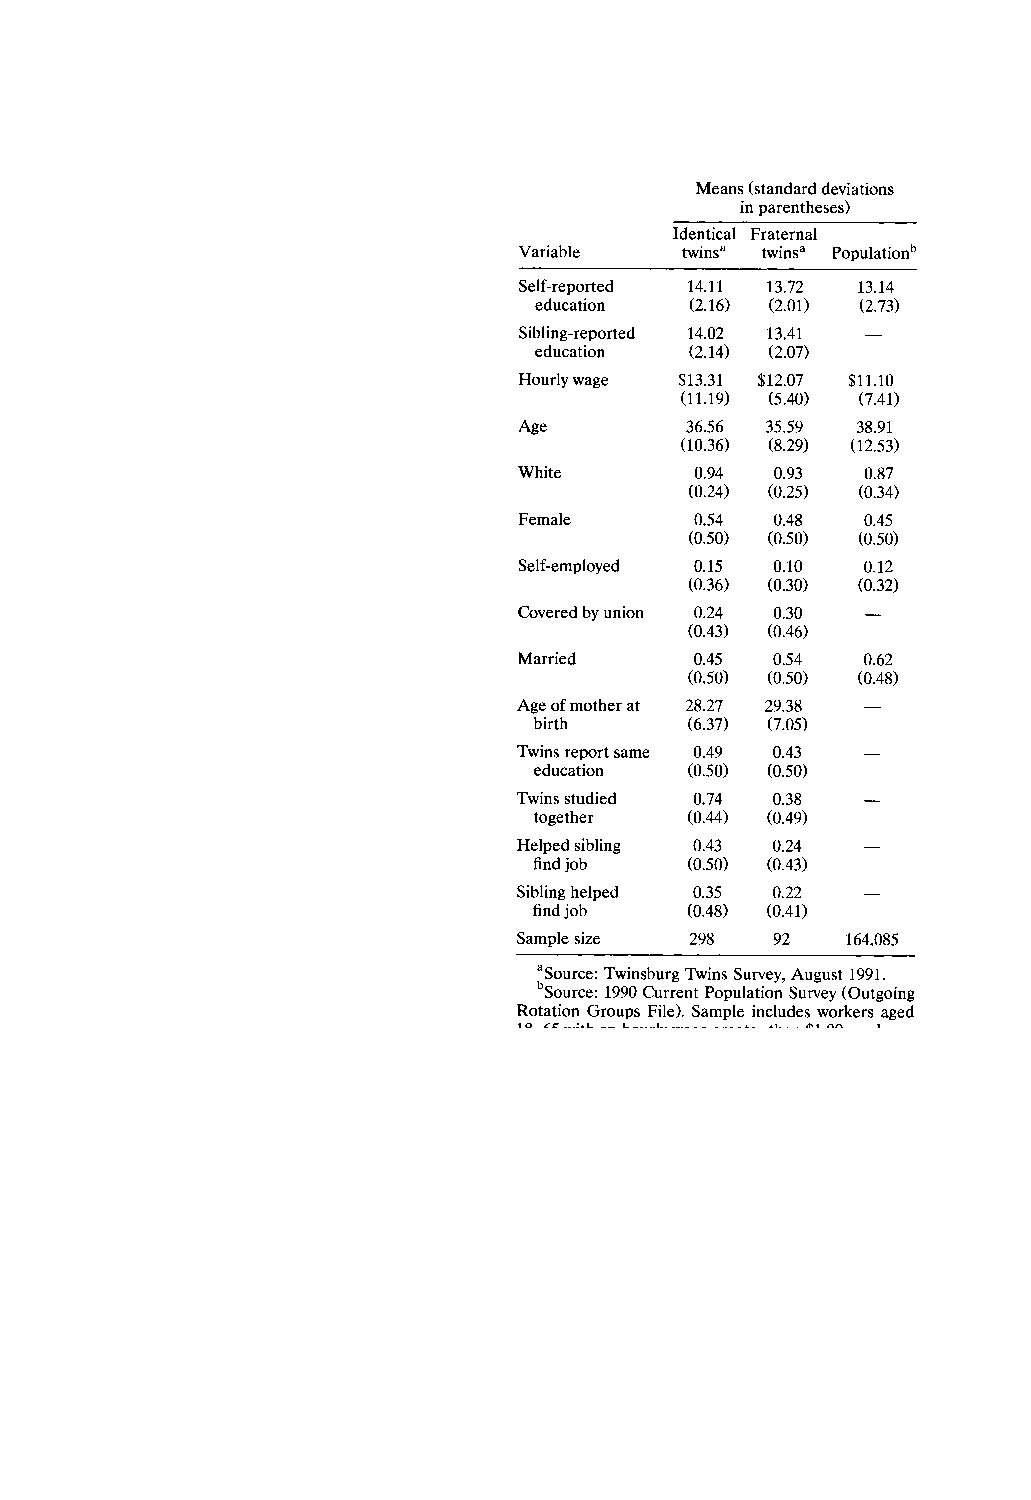
\includegraphics[width=0.4\linewidth]{graphs/ashenfelter_krueger_tab1.pdf}
\end{figure}
\end{center}
 }


\begin{frame}
\frametitle{Is there measurement error?}

Classical ME assumptions:
\begin{eqnarray*}
s^{j}_{k} &=& s^{*}_{k}+ \epsilon^{j}_{k},  \;\;\;j, k=1, 2 \\
Cov(s^{*}_{k}, \epsilon^{j}_{k})&=& Cov(s^{*}_{k}, \epsilon^{k}_{j}) =Cov( \epsilon^{j}_{k}, \epsilon^{k}_{j}) = 0 \\
\end{eqnarray*}
To check correlations
\begin{eqnarray*}
Corr(s^{1}_{1}, s^{2}_{1})&=& \frac{Var(s^{*}_{1})}{\sqrt{Var(s^{1}_{1})Var(s^{2}_{1})}} \\
                                     &=& 1-\frac{\sigma^{2}_{\epsilon}}{\sigma^{2}_{s}}=\underbrace{1-\lambda}_{\text{reliability ratio}} 
\end{eqnarray*}
\begin{itemize}
\item $Corr(s^{1}_{1}, s^{2}_{1})=0.92$, $Corr(s^{2}_{2}, s^{1}_{2})=0.88$ in Table 2

\item 8-12\% in the measured variance in schooling levels is error

\item Measurement error in parental schooling levels


$EF= 0.86$, father, $EM= 0.84$



\end{itemize}
\end{frame}

\frame{ \frametitle{}
\begin{center}
\begin{figure}[t]
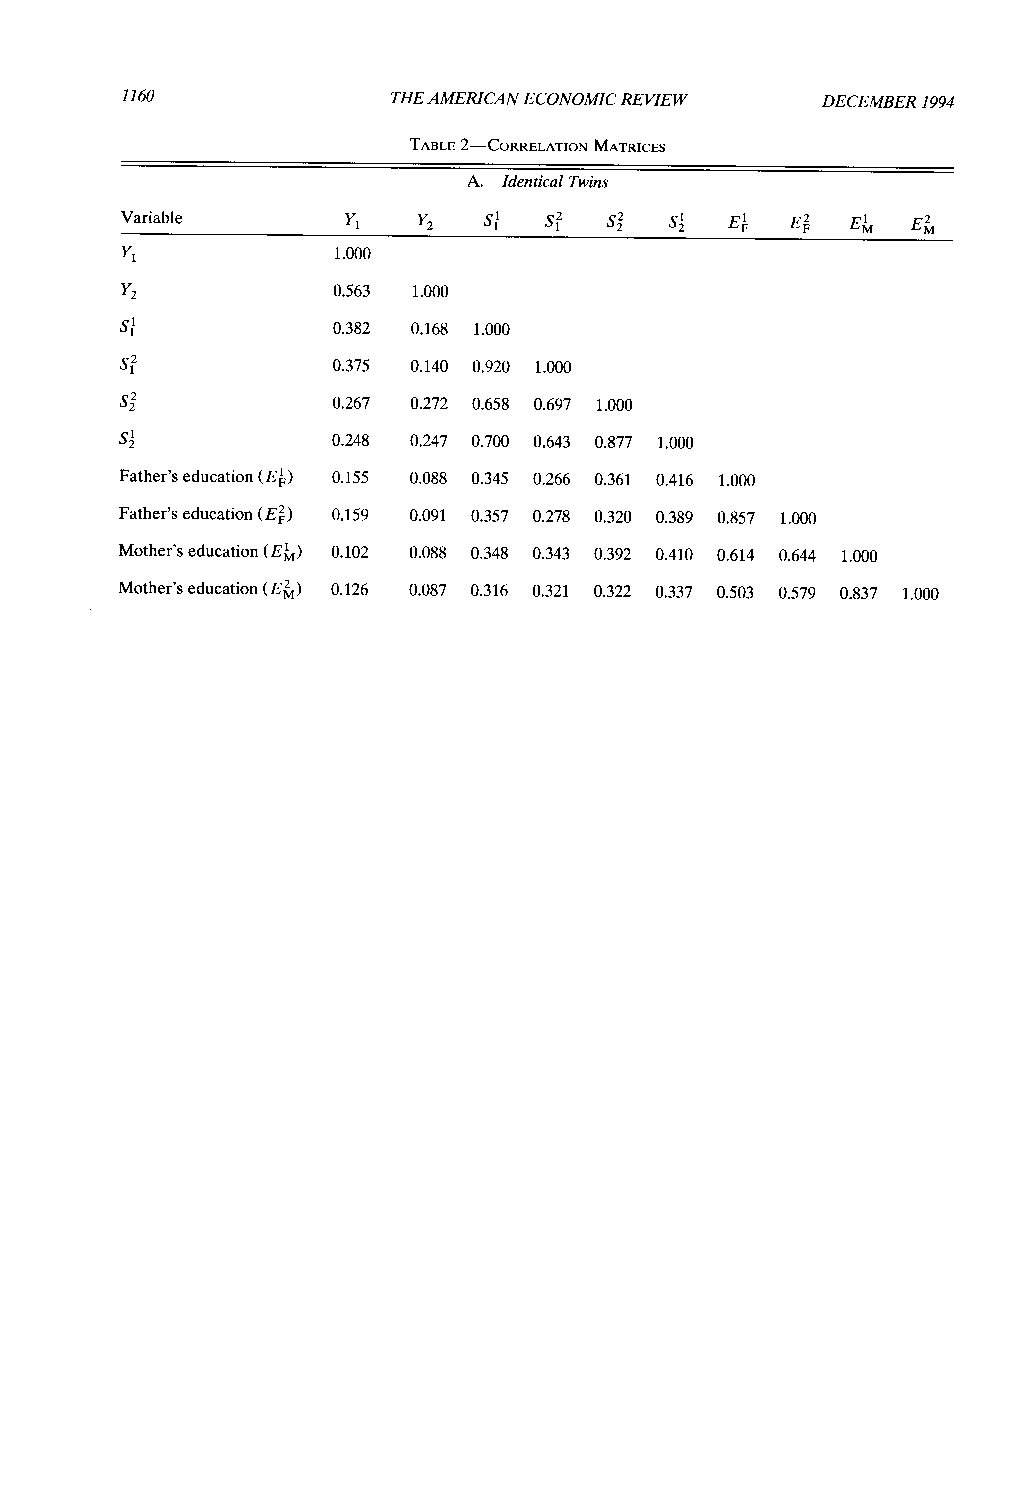
\includegraphics[width=1.0\linewidth]{graphs/ashtab2.pdf}
\end{figure}
\end{center}
 }
 
 

\begin{frame}
\frametitle{First difference model}

\begin {itemize}
    \item  $Y_{1i}$, log wage twin 1
    \item $Y_{2i}$, log wage twin 2
    \item $X_{i}$, variables that vary by family
    \item $s_{1i}, s_{2i}$ schooling

 \begin{eqnarray*}
     Y_{1i} &=& \alpha+ \rho s_{1i}+ X^{'}_{i}\beta+u_{1i}+ A^{'}_{i}\gamma\\
     Y_{2i} &=& \alpha+ \rho s_{2i}+ X^{'}_{i}\beta+u_{2i}+ A^{'}_{i}\gamma
\end{eqnarray*}
\item Difference:
\begin{eqnarray*}
     Y_{1i} -Y_{2i}=  \rho \left(s_{1i}-s_{2i}\right)+ u_{1i}-u_{2i}
     \end{eqnarray*}
\item Fixed effects estimator, $A_{i}$ eliminated by differencing
\end {itemize}
\end{frame}



\frame{ \frametitle{}
\begin{center}
\begin{figure}[t]
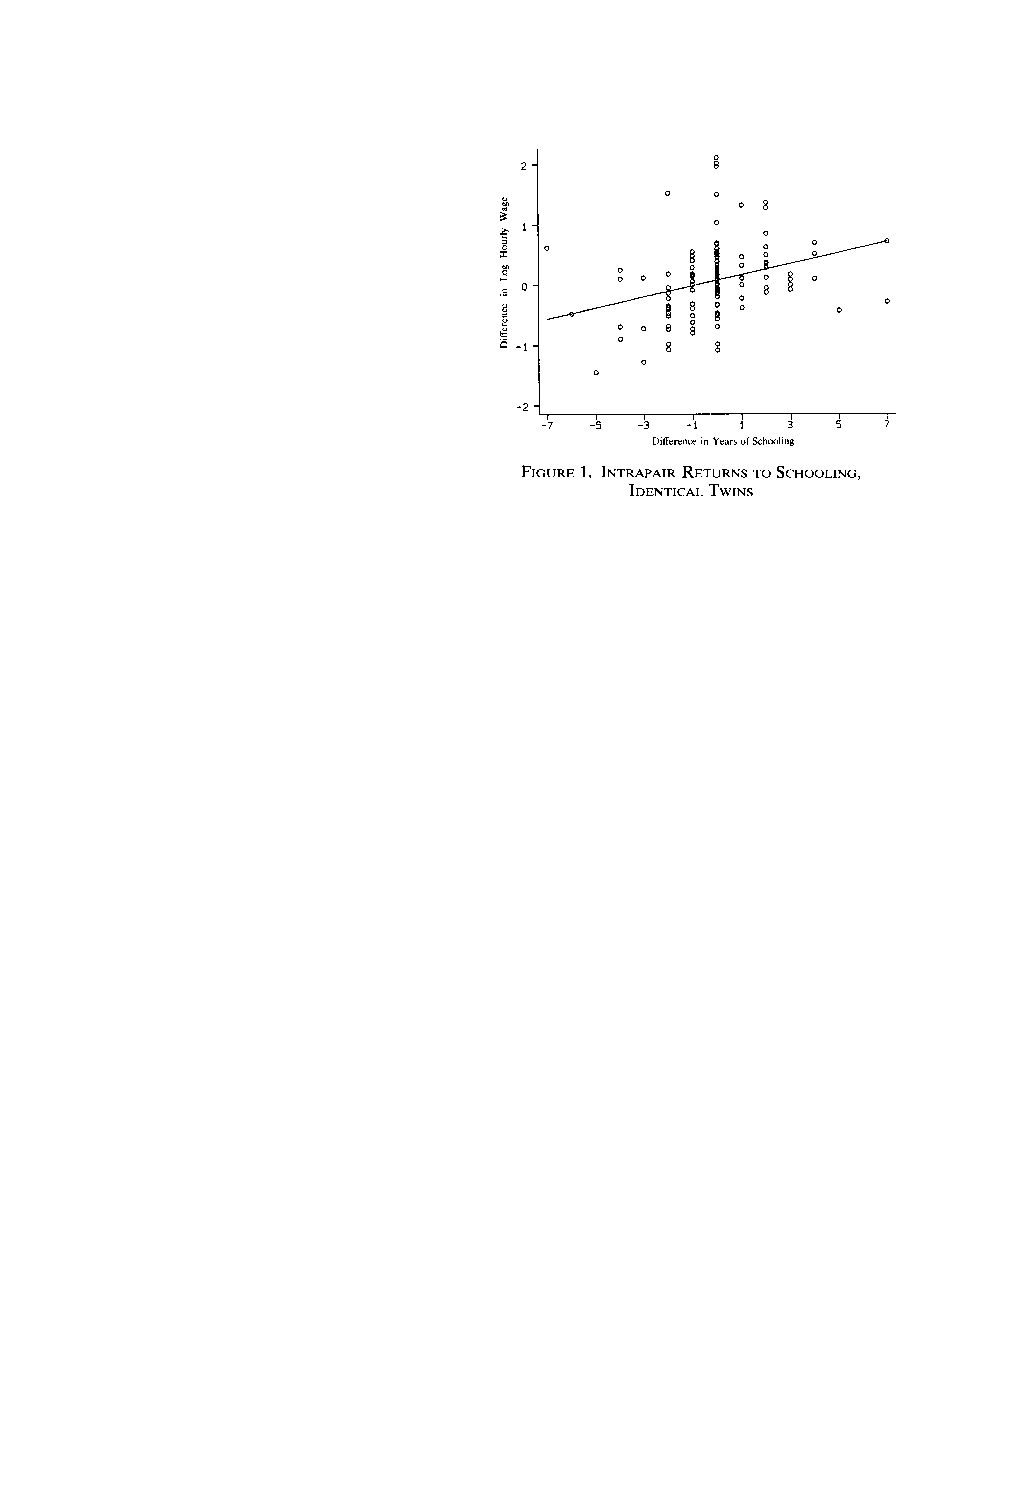
\includegraphics[width=1.0\linewidth]{graphs/ashfig1.pdf}
\end{figure}
\end{center}
 }



% Slide 11

\begin{frame}
\frametitle{Measurement error}
\begin{itemize}
\item Measurement error in $s$

\begin{eqnarray*}
  s_{1i}&=& s^{*}_{1i}+ \epsilon_{1i}\\
   s_{2i}&=& s^{*}_{2i}+ \epsilon_{2i}
\end{eqnarray*}


\item Classical ME:
   \begin{eqnarray*}
  Cov\left(s^*_{1i}, \epsilon_{1i}\right)&=&0\\
  Cov\left(s^*_{2i}, \epsilon_{2i}\right)&=&0\\
  Cov\left(s^*_{1i}, \epsilon_{2i}\right)&=&  Cov\left(s^*_{2i}, \epsilon_{1i}\right)= 0\\
   Cov\left(\epsilon_{1i}, \epsilon_{2i}\right)&=&0
\end{eqnarray*}
\end {itemize}
\end{frame}


% slide 12

\begin{frame}
\frametitle{Measurement error bias}
\begin{itemize}
\item Differenced equation:
   \begin{eqnarray*}
       Y_{1i} -Y_{2i}=  \rho \left(s^{*}_{1i}-s^{*}_{2i}\right) +u_{1i}-u_{2i}
\end{eqnarray*}

\item Estimated equation
\begin{eqnarray*}
       Y_{1i} -Y_{2i}&=&  \rho \left(s_{1i}-s_{2i}\right) +u_{1i}-u_{2i} + \rho \left(\epsilon_{1i}-\epsilon_{2i}\right)
\end{eqnarray*}
\item Bias
\begin{eqnarray*}
       \tilde{\rho}&=&\rho \left(1- \frac{\sigma^{2}_{\epsilon}}{\sigma^{2}_{s^{*}}+\sigma^{2}_{\epsilon}}\frac{1}{1-r_{s}}\right)\\
       &=& \rho\left(1-\lambda\frac{1}{1-r_{s}}\right)
\end{eqnarray*}

\item $r_{s}$ within family correlation in schooling levels
\item Differencing takes out a lot of the signal, but not the noise
\end{itemize}
\end{frame}



%slide 13
\begin{frame}
\frametitle{Approximation of attenuation bias}

\begin{eqnarray*}
       \tilde{\rho}    &=& \rho\left(1-\lambda\frac{1}{1-r_{s}}\right)
\end{eqnarray*}

From Table 2:
\begin{itemize}
\item $\lambda=0.1$

\item $r_{s}=0.66$.

\item  Bias is $\frac{0.1}{1-0.66}\approx30\%$

\end{itemize}

\end{frame}


%slide 15

\begin{frame}
\frametitle{Simple OLS procedure to deal with measurement error}
\begin{itemize}
\item Use average over multiple education reports $(\frac{s^{1}_{1}+ s^{2}_{1}}{2} ) - (\frac{s^{1}_{2}+s^{1}_{2}}{2}) $ 



\item Averaging decreases measurement error as a fraction of total variance.

\begin{eqnarray*}
\tilde{\rho}=\rho \left(1- \frac{\lambda}{1-r_{s}}-\frac{2Var(s^*_{1}-s^*_{2})}{2}\right)
\end{eqnarray*}

\end{itemize}

\end{frame}


\begin{frame}
\frametitle{Instrumental variables strategy}

\begin{itemize}

\item Get another measure on $s^{*}_{i} $ from an independent source 

\item Ask \emph{twin 2} about \emph{twin 1} schooling and vice versa

\item $s^{k}_{j} $, $j=1,2$  and $k=1,2$
\item  $s^{1}_{1} $, $s^{2}_{2} $ self reports

\item  $s^{2}_{1} $, $s^{1}_{2} $ cross reports

\item All measures are highly correlated (see Table 2)

\end{itemize}

\end{frame}











%slide 16

\begin{frame}
\frametitle{IV Procedure}
\begin{itemize}
\item Independent measure of schooling as instrument

\begin{eqnarray*}
Y_{1}-Y_{2}= \rho\left(s^1_{1}-s^2_{2}\right)+ \underbrace{\left(u_{1}-u_{2}\right)+\left(\epsilon^1_{1}-\epsilon^2_{2}\right)}_{v_{1}-v_{2}}
\end{eqnarray*}


 \item Use independent measures of $s^*_{j}$ to construct an instrument for $(s^1_{1}-s^2_{2})$
\begin{equation*}
    z=(s^2_{1}-s^1_{2})
\end{equation*}

\item Exclusion restriction: $z_{i}$ uncorrelated with $\left(v_{1i}-v_{2i}\right)$ .
\item Relevance: $z_{i}$ correlated  with $\left(s^*_{1i}-s^*_{2i}\right)$



\end{itemize}

\end{frame}


\frame{ \frametitle{}
\begin{center}
\begin{figure}[t]
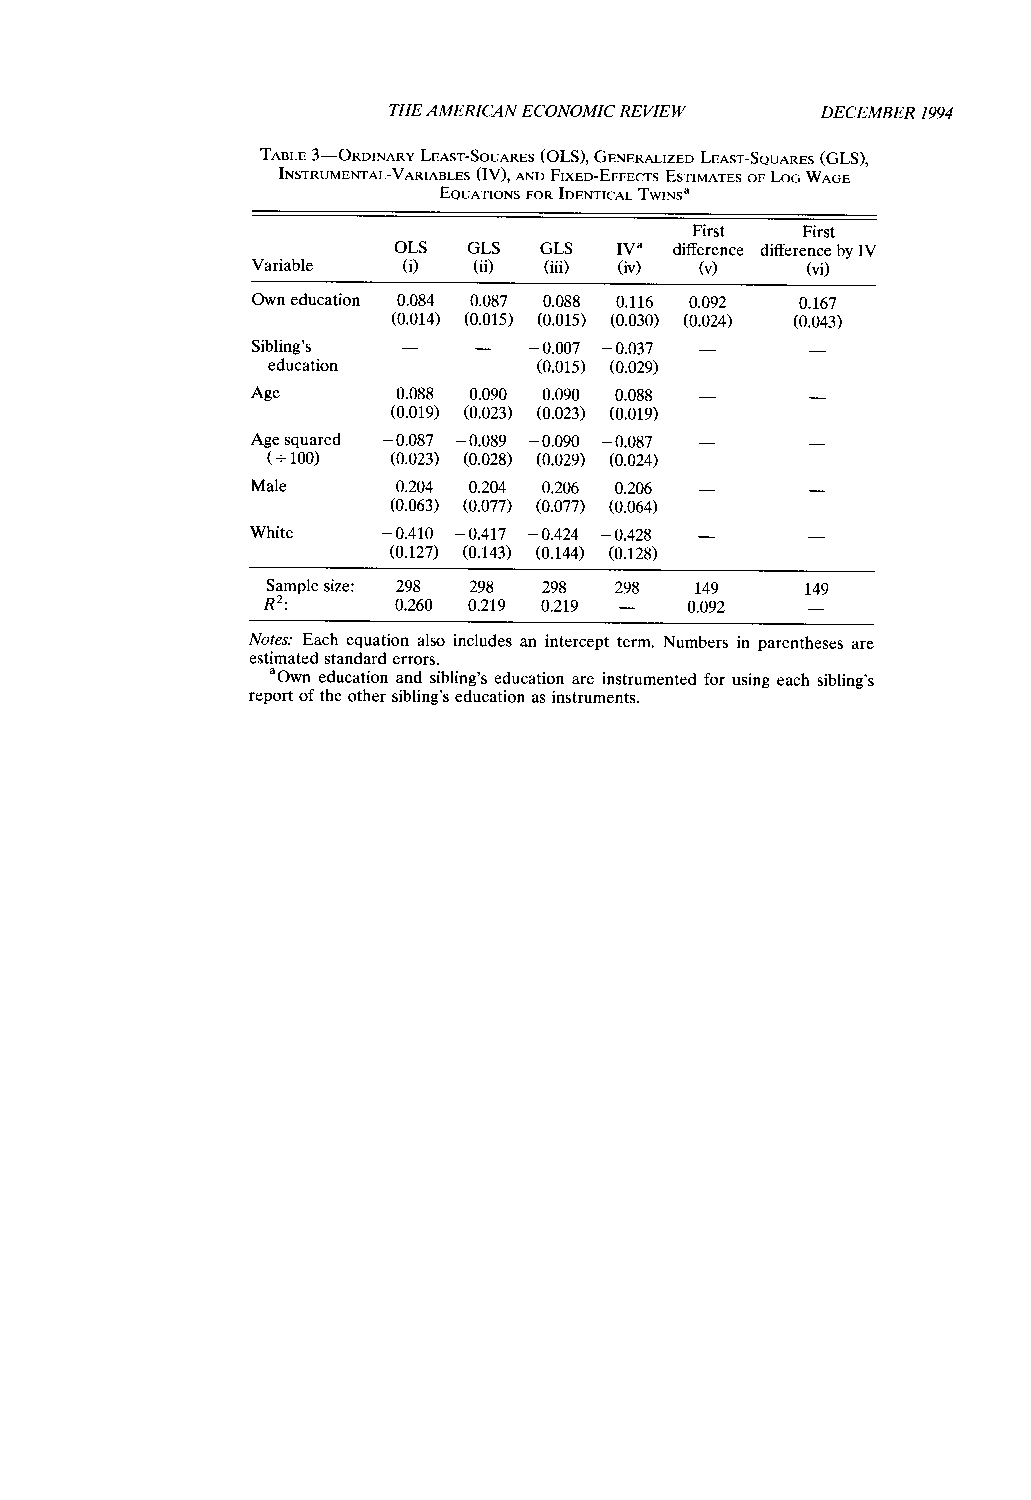
\includegraphics[width=1.0\linewidth]{graphs/ashtab3.pdf}
\end{figure}
\end{center}
 }





 \frame{ \frametitle{}
\begin{center}
\begin{figure}[t]
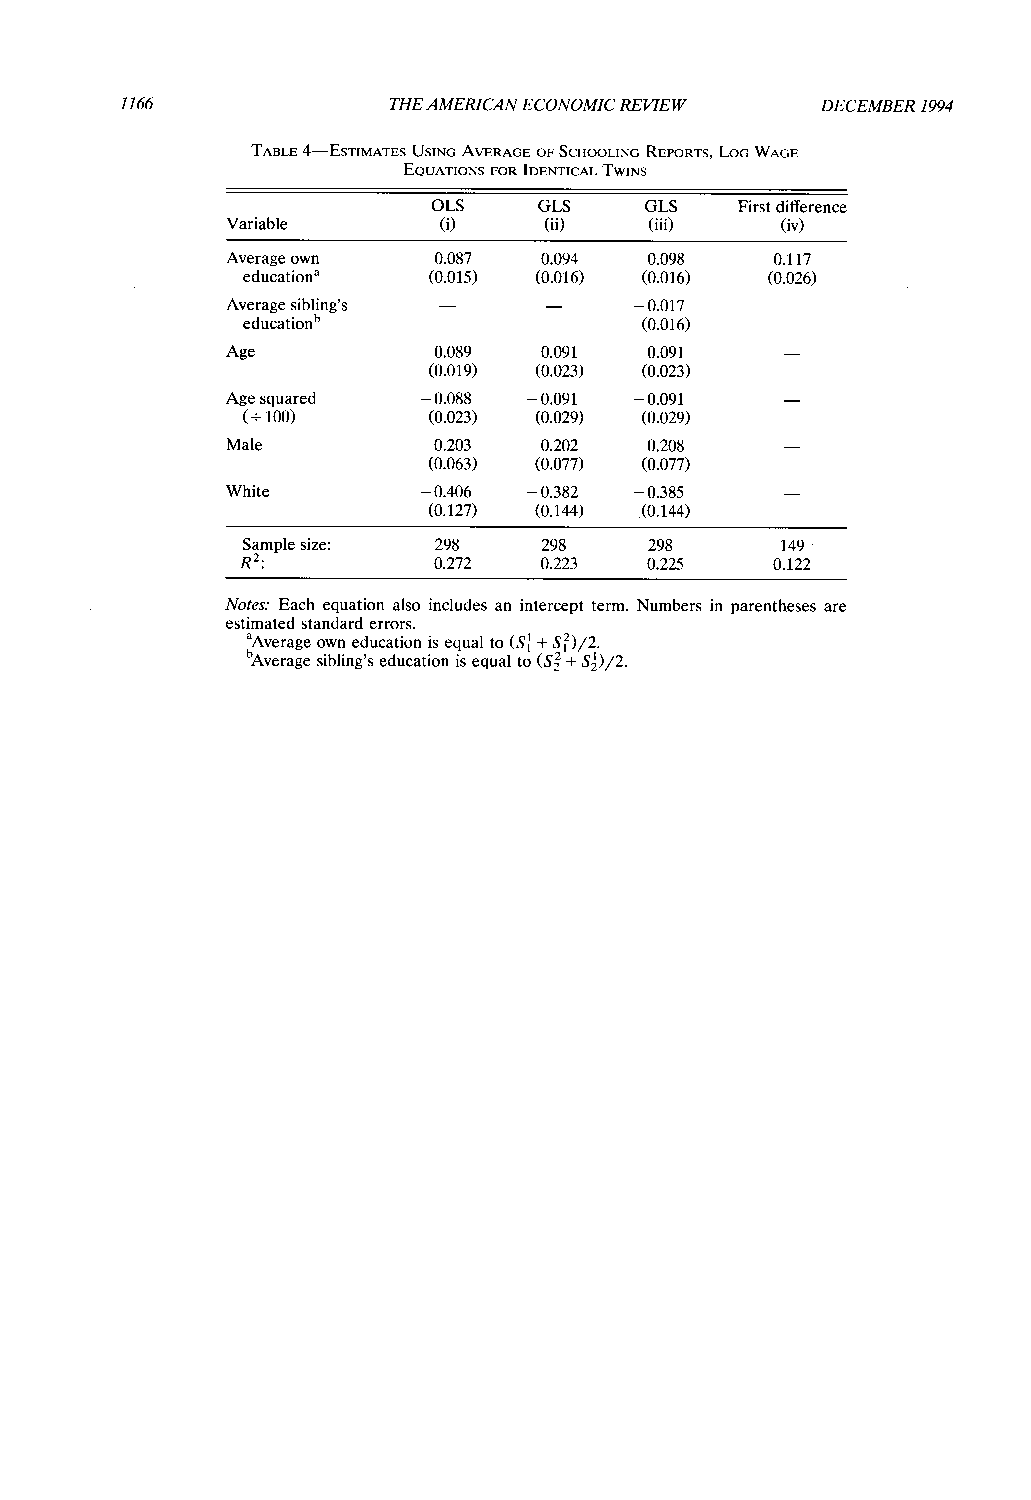
\includegraphics[width=1.0\linewidth]{graphs/ashtab4.pdf}
\end{figure}
\end{center}
 }




\frame{ \frametitle{}
\begin{center}
\begin{figure}[t]
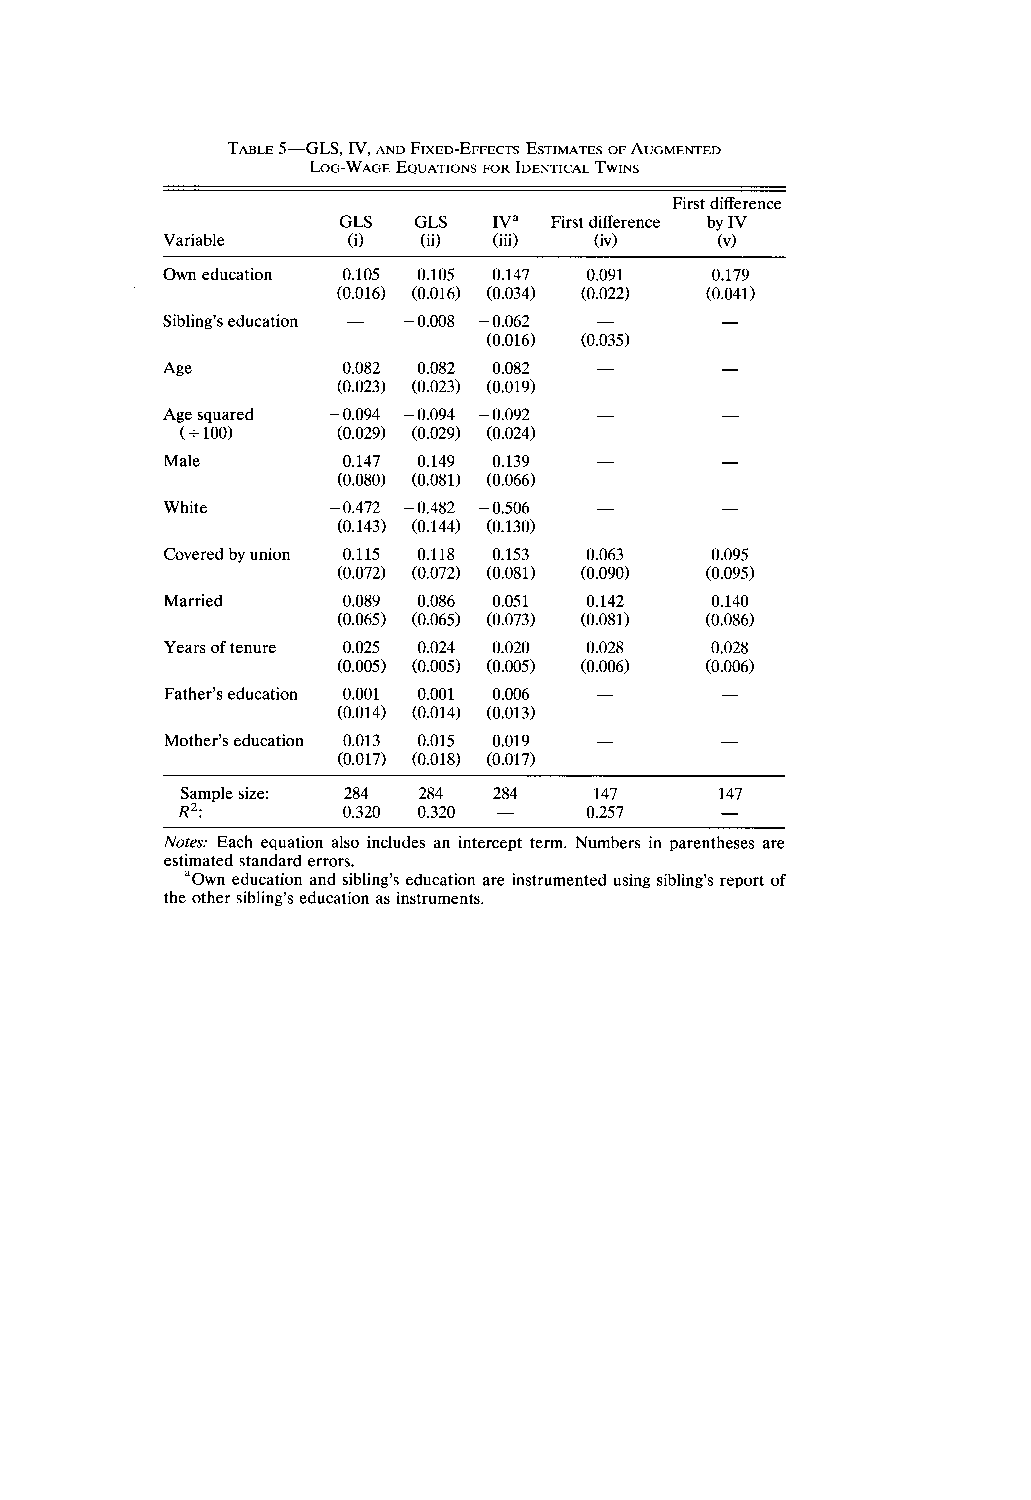
\includegraphics[width=0.7\linewidth]{graphs/ashenfelter_krueger_tab5.pdf}
\end{figure}
\end{center}
 }



  \frame{ \frametitle{Correlated measurement error}

  Individuals who report upward biased measure of own education may be more likely to report upward biased education for their sibling
   \begin{equation*}
 \rho_{v} = corr(\epsilon^1_{1},\epsilon^1_{2}) = corr(\epsilon^2_{1},\epsilon^2_{2}) >0
\end{equation*}
\begin{itemize}
  \item this implies that $s^1_{1}$ and $s^1_{2}$ are more strongly correlated than $s^1_{1}$ and $s^2_{2}$, see Table 2
  \item the previous IV strategy fails, because
  \[ cov(s^*_{1}-s^*_{2}+(\epsilon^1_{1}-\epsilon^2_{2}), (u_{1}- u_{2}) +(\epsilon^2_{1}-\epsilon^1_{2}))\neq 0 \]
\end{itemize}
rewrite the model
 \begin{equation*}
  Y_{1}-Y_{2} = \delta (s^1_{1}-s^1_{2})+ \tilde{\varepsilon}
\end{equation*}
and use $z=s^2_{1}-s^2_{2}$ as an instrument

}


\frame{ \frametitle{}
\begin{center}
\begin{figure}[t]
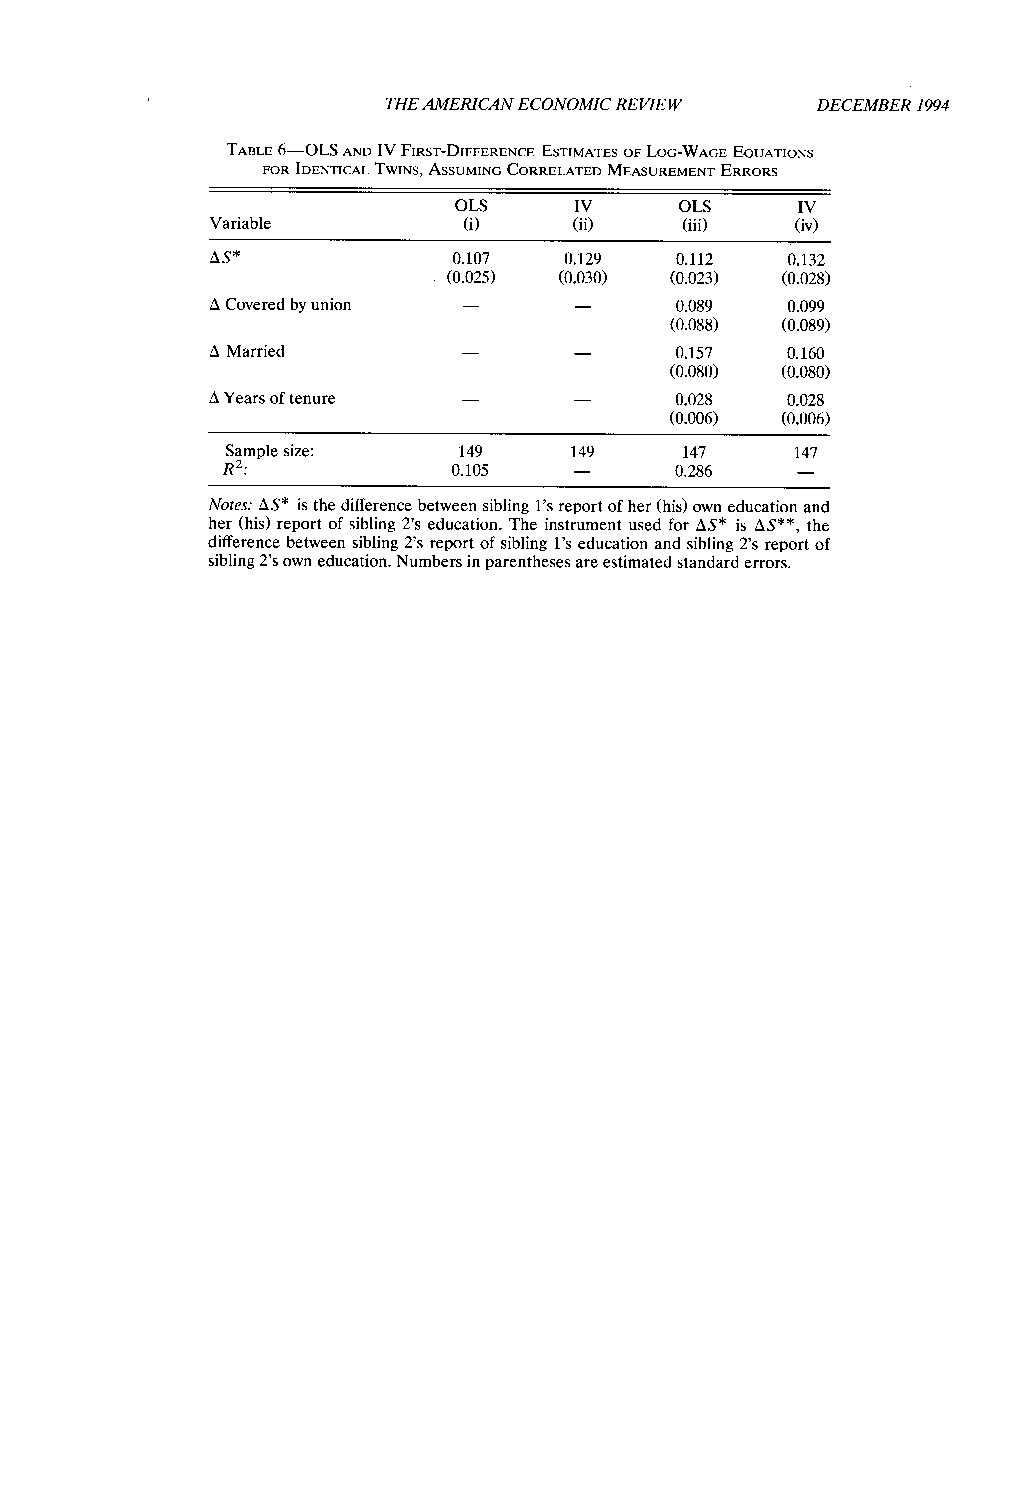
\includegraphics[width=1.0\linewidth]{graphs/ashtab6.pdf}
\end{figure}
\end{center}
 }

 \frame{ \frametitle{Book References}
\begin{itemize}
\item Angrist, Joshua D., and J\"{o}rn-Steffen Pischke. Mastering' metrics: The path from cause to effect. Princeton University Press, 2014.
\item Wooldridge, pages 318-324
\end{itemize}
}
 \end{document}



\end {document} 